\documentclass[]{elsarticle} %review=doublespace preprint=single 5p=2 column
%%% Begin My package additions %%%%%%%%%%%%%%%%%%%
\usepackage[hyphens]{url}

  \journal{SportR\(\chi\)iv} % Sets Journal name


\usepackage{lineno} % add

\usepackage{graphicx}
%%%%%%%%%%%%%%%% end my additions to header

\usepackage[T1]{fontenc}
\usepackage{lmodern}
\usepackage{amssymb,amsmath}
\usepackage{ifxetex,ifluatex}
\usepackage{fixltx2e} % provides \textsubscript
% use upquote if available, for straight quotes in verbatim environments
\IfFileExists{upquote.sty}{\usepackage{upquote}}{}
\ifnum 0\ifxetex 1\fi\ifluatex 1\fi=0 % if pdftex
  \usepackage[utf8]{inputenc}
\else % if luatex or xelatex
  \usepackage{fontspec}
  \ifxetex
    \usepackage{xltxtra,xunicode}
  \fi
  \defaultfontfeatures{Mapping=tex-text,Scale=MatchLowercase}
  \newcommand{\euro}{€}
\fi
% use microtype if available
\IfFileExists{microtype.sty}{\usepackage{microtype}}{}
\usepackage[margin=1in]{geometry}
\bibliographystyle{elsarticle-harv}
\ifxetex
  \usepackage[setpagesize=false, % page size defined by xetex
              unicode=false, % unicode breaks when used with xetex
              xetex]{hyperref}
\else
  \usepackage[unicode=true]{hyperref}
\fi
\hypersetup{breaklinks=true,
            bookmarks=true,
            pdfauthor={},
            pdftitle={Determining optimal shot selection strategy in Super Netball's `Power 5' period via numerical simulation},
            colorlinks=false,
            urlcolor=blue,
            linkcolor=magenta,
            pdfborder={0 0 0}}
\urlstyle{same}  % don't use monospace font for urls

\setcounter{secnumdepth}{0}
% Pandoc toggle for numbering sections (defaults to be off)
\setcounter{secnumdepth}{0}


% tightlist command for lists without linebreak
\providecommand{\tightlist}{%
  \setlength{\itemsep}{0pt}\setlength{\parskip}{0pt}}


% Pandoc citation processing
\newlength{\cslhangindent}
\setlength{\cslhangindent}{1.5em}
\newlength{\csllabelwidth}
\setlength{\csllabelwidth}{3em}
\newlength{\cslentryspacingunit} % times entry-spacing
\setlength{\cslentryspacingunit}{\parskip}
% for Pandoc 2.8 to 2.10.1
\newenvironment{cslreferences}%
  {}%
  {\par}
% For Pandoc 2.11+
\newenvironment{CSLReferences}[2] % #1 hanging-ident, #2 entry spacing
 {% don't indent paragraphs
  \setlength{\parindent}{0pt}
  % turn on hanging indent if param 1 is 1
  \ifodd #1
  \let\oldpar\par
  \def\par{\hangindent=\cslhangindent\oldpar}
  \fi
  % set entry spacing
  \setlength{\parskip}{#2\cslentryspacingunit}
 }%
 {}
\usepackage{calc}
\newcommand{\CSLBlock}[1]{#1\hfill\break}
\newcommand{\CSLLeftMargin}[1]{\parbox[t]{\csllabelwidth}{#1}}
\newcommand{\CSLRightInline}[1]{\parbox[t]{\linewidth - \csllabelwidth}{#1}\break}
\newcommand{\CSLIndent}[1]{\hspace{\cslhangindent}#1}

\usepackage{booktabs}
\usepackage{longtable}
\usepackage{array}
\usepackage{multirow}
\usepackage{wrapfig}
\usepackage{float}
\usepackage{colortbl}
\usepackage{pdflscape}
\usepackage{tabu}
\usepackage{threeparttable}
\usepackage{threeparttablex}
\usepackage[normalem]{ulem}
\usepackage{makecell}
\usepackage{xcolor}



\begin{document}


\begin{frontmatter}

  \title{Determining optimal shot selection strategy in Super Netball's
`Power 5' period via numerical simulation}
    \author[Centre for Sport Research]{Aaron S. Fox\corref{1}}
  
    \author[Centre for Sport Research]{Tanisha Bardzinski}
  
    \author[Centre for Sport Research]{Lyndell Bruce}
  
      \address[Centre for Sport Research]{Centre for Sport Research,
School of Exercise and Nutrition Sciences, Deakin University, Geelong,
Australia}
      \cortext[1]{Corresponding Author: aaron.f@deakin.edu.au}
  
  \begin{abstract}
  Insert abstract\ldots{}
  \end{abstract}
  
 \end{frontmatter}

\hypertarget{todo}{%
\section{TODO:}\label{todo}}

\begin{itemize}
\tightlist
\item
  Check consistency of Super Shot vs.~Power 5 period (use Power 5
  period)
\item
  Look to ESSA abstract for some sample points and language
\item
  Add line spacing between paragraphs
\end{itemize}

\hypertarget{introduction}{%
\section{Introduction}\label{introduction}}

Netball is a court-based team sport played predominantly among
Commonwealth nations, and has one of the highest participation rates for
team sports in Australia (\textbf{AustralianSportsCommission2020?}). As
in many court-based team sports, the goal of netball is to score more
than the opposition. Netball is, however, unique in that goals may only
be scored by two players on each team from within the `shooting circle'
(i.e.~a half circle around the goal with a 4.9m radius) at their end of
the court (\textbf{INFrules?}). Traditionally, goals scored from within
this circle result in one goal for the team (\textbf{INFrules?}). In the
2020 season, Australia's national elite-level league (i.e.~Suncorp Super
Netball) made the decision to introduce the `Super Shot'
(\textbf{NetballAusSuperShotIntro?}). The Power 5 provided teams an
opportunity to gain one- versus two-goals for successful shots made from
the `inner' (i.e.~0m-3.0m) versus `outer' (i.e.~3.0m-4.9m) circles,
respectively, within the final five minutes of each quarter (i.e.~the
Power 5 period) (\textbf{NetballAusSuperShotIntro?}). The rule has
remained in place over subsequent seasons since the 2020 inception.

Our analysis prior to the 2020 season (\textbf{Fox2020?}) suggested that
the added value of the Super Shot (i.e.~two-goals) aligned well with the
elevated risk of shooting from long range, and that teams may have been
able to maximise their scoring by taking a high proportion of Super
Shots. These findings were, however, based on shooting statistics from a
past season where the Super Shot rule was not in effect. Further
investigation of netball competitions where a `two-goal rule' was in
place (i.e.~international Fast5) resulted in a much higher risk of
missing long-range shots (\textbf{Fox2020?}). We hypothesised that the
elevated risk of missing long-range shots with a `two-goal rule' in
place stems from situational factors, whereby defensive strategies were
likely altered to place a heavier emphasis on defending long-range shots
(\textbf{Fox2020?}). Data from the early years of the Super Shot in
place provides an opportunity to re-evaluate the risk:reward value of
taking Super Shots with more valid shooting statistics. Further, these
data can provide a better foundation for simulating Power 5 periods as a
means to identify optimal shooting strategies. In the present study, we
first ran simulations of the Power 5 period for each team individually
in an attempt to identify expected scoring outcomes stemming from
different Super Shot selection strategies. Second, we ran simulations of
teams competing against one another during a Power 5 period to determine
how varying the Super Shot selection strategy could impact scoring
margin.

\hypertarget{methods}{%
\section{Methods}\label{methods}}

\hypertarget{participants}{%
\subsection{Participants}\label{participants}}

Participants for this study included all players across the eight teams
from the 2020-2022 seasons season of the Australian national netball
league (i.e.~Suncorp Super Netball). Our study included publicly
available, pre-existing data held on the Suncorp Super Netball Match
Centre. An exemption from ethics review was granted by the Deakin
University Human Research Ethics Committee (\textbf{\emph{TODO: add
details}}).

\hypertarget{data-collection}{%
\subsection{Data Collection}\label{data-collection}}

We used the \emph{\{SuperNetballR\}} (\textbf{\emph{TODO: citation}})
package to extract match data from all regular season games during the
2020-2022 Super Netball Seasons via the Champion Data (official provider
of competition statistics) Match Centre. All shots are labelled with
identifiers that place them in the inner or outer circle, along with
whether they were made or missed. Combined with the timestamp of these
events within quarters, we extracted team-specific shooting statistics
for: (i) the total number of shots taken; (ii) the number of shots taken
from the inner and outer circle; and (iii) the number of made and missed
shots from the inner and outer circle from each Power 5 period across
matches.

\hypertarget{data-analysis}{%
\subsection{Data Analysis}\label{data-analysis}}

Our study required estimating the probability of making versus missing
shots from the inner versus outer circle across the different teams. We
achieved this by defining a beta distribution in a probability density
function for the different circle zones, specified by:

\[f(x,a,b) = \frac{\Gamma(a+b)x^{a-1}(1-x)^{b-1}}{\Gamma(a)\Gamma(b)} \]
where \(a\) and \(b\) represent the number of missed and made shots
within a circle zone, respectively; \(x\) is the probability of \(a\)
relative to \(b\); and \(\Gamma\) is the gamma function
(\textbf{NIST2020?}). Probability density functions were created for
made versus missed shots in the inner and outer circles for each team to
be used in subsequent simulations.

First --- we ran a series of simulations (\emph{n} = 1,000 each) of the
Power 5 period for each team, altering the `tendency' for each shot to
be taken as a Super Shot. Across each individual simulation, the total
number of shots the team received was driven by their expected number of
shots in a Power 5 period based on the three seasons worth of data.
Specifically, the mean and standard deviation (SD) of shots a team took
during Power 5 periods was used to create a truncated normal
distribution (upper and lower limits set at ±95\% confidence intervals
{[}CIs{]}) --- of which the number of shots for a team in an individual
simulation were randomly sampled from. Within each simulation, whether
an individual shot was taken as a standard or Super Shot was dictated by
the current tendency being simulated. We repeated each simulation across
five tendencies towards taking Super Shots, those being: (i) `zero' (0\%
chance of Super Shot being taken); (ii) `low' (25\% chance of Super Shot
being taken); (iii) `moderate' (50\% chance of Super Shot being taken);
(iv) `high' (75\% chance of Super Shot being taken); and (v) `all out'
(100\% chance of Super Shot being taken). For each individual shot
during the simulation, a random number between zero and one was
generated from a uniform distribution --- and a Super versus standard
shot was taken depending on if this was lower versus higher,
respectively, than the chance of taking a Super Shot (e.g.~a random
value of 0.45 within a `high' tendency simulation would result in a
Super Shot being taken). The success (i.e.~make vs.~miss) of each
individual standard or Super Shot within the simulation was then
determined by generating a random value between zero and one from a
uniform distribution, alongside a value sampled from the teams relevant
probability density function of making a shot from the relevant location
(i.e.~inner or outer circle). If the value sampled from the probability
density function was greater versus lower than the random value --- the
shot was considered successful versus unsuccessful, respectively. After
all individual shots were simulated, the total team score was summed
given the value of the made standard and Super shots. We calculated the
scores achieved with the varying Super Shot tendencies relative to the
`zero' tendency (mean ± SD, range) to examine the expected increase or
decrease in scoring with altered Super Shot selection strategies.

A similar approach was taken in simulating teams competing against one
another during Power 5 periods. A series of simulations (\emph{n} =
1,000) of Power 5 periods were ran between all combinations of teams. We
once again used the probabilities of making versus missing shots from
within and outside the outer circle during the Power 5 period from each
team to estimate scoring. To determine the number of shots each team
received in a simulation, we created two truncated normal distributions
based on the mean and SD of total shots of total shots and the
proportion of shots by teams in Power 5 periods (upper and lower limits
set at minimum and maximum values). The number of shots the first team
received (i.e.~Team A) was determined by the product of values randomly
sampled from the two distributions (e.g.~values of 12 and 0.75 would
result in 9 shots to Team A) distribution of total shots. The number of
shots the second team received (i.e.~Team B) was then determined by
allocating those remaining from the total shots (e.g.~in the
aforementioned example Team B would receive the remaining 3 shots). As
part of this approach we ensured that there was an appropriate balance
between the disparity if shots each team received (i.e.~each team
received an even amount of simulations where they had the same amount of
more vs.~less shots). The series of 1,000 simulations was repeatedly ran
between all combinations of teams and the aforementioned Super Shot
selection tendencies. Standard versus Super Shot selection and shot
success within simulations were determined in the same manner described
earlier (i.e.~random number generator vs.~chance of Super Shot being
taken and value sampled from the teams shot success probability
distribution). At the end of each simulation, the teams scores were
summed and the subsequent margin determined. The mean ± SD and range for
margins between each team across the various Super Shot tendency
combinations were then calculated. We also inspected the proportion of
simulations each team won versus lost across simulations and the mean ±
SD margin in these cases.

\hypertarget{results}{%
\section{Results}\label{results}}

The shot frequencies for each team used to create probability density
functions for use in simulations are displayed in Table
\ref{tab:shotFrequencyTable}.

\begin{table}

\caption{\label{tab:shotFrequencyTable}Shot frequencies by team across 2020 — 2022 seasons used to create probability density functions for use in simulations.}
\centering
\begin{tabular}[t]{lrrrr}
\toprule
Team & Standard Goal & Standard Miss & Super Shot Goal & Super Shot Miss\\
\midrule
Fever & 783 & 24 & 168 & 159\\
Firebirds & 622 & 87 & 179 & 207\\
GIANTS & 409 & 37 & 315 & 254\\
Lightning & 634 & 68 & 162 & 152\\
Magpies & 590 & 47 & 159 & 140\\
\addlinespace
Swifts & 545 & 62 & 201 & 176\\
Thunderbirds & 527 & 48 & 167 & 170\\
Vixens & 527 & 60 & 194 & 176\\
\bottomrule
\end{tabular}
\end{table}

Our initial simulations of individual team scoring within Power 5
periods using variable Super Shot selection tendencies found a small
increase in mean scoring relative to the `zero' Super Shot tendency.
Across all teams, the mean (± SD) goals scored relative to the `zero'
tendency was 1.03 (± 0.21), 1.07 (± 0.30), 1.10 (± 0.37) and 1.14 (±
0.43) across the `low,' `moderate,' `high' and `all out' strategies,
respectively. Alongside the mean increase in relative goals scored, we
observed a corresponding widening of the variance (i.e.~SD) and range of
scoring values (i.e.~range) with higher tendencies to take Super Shots
--- with these observations consistent across teams (see Figure
\ref{fig:standardSimsRelativeGoalsScored}).

\begin{figure}

{\centering 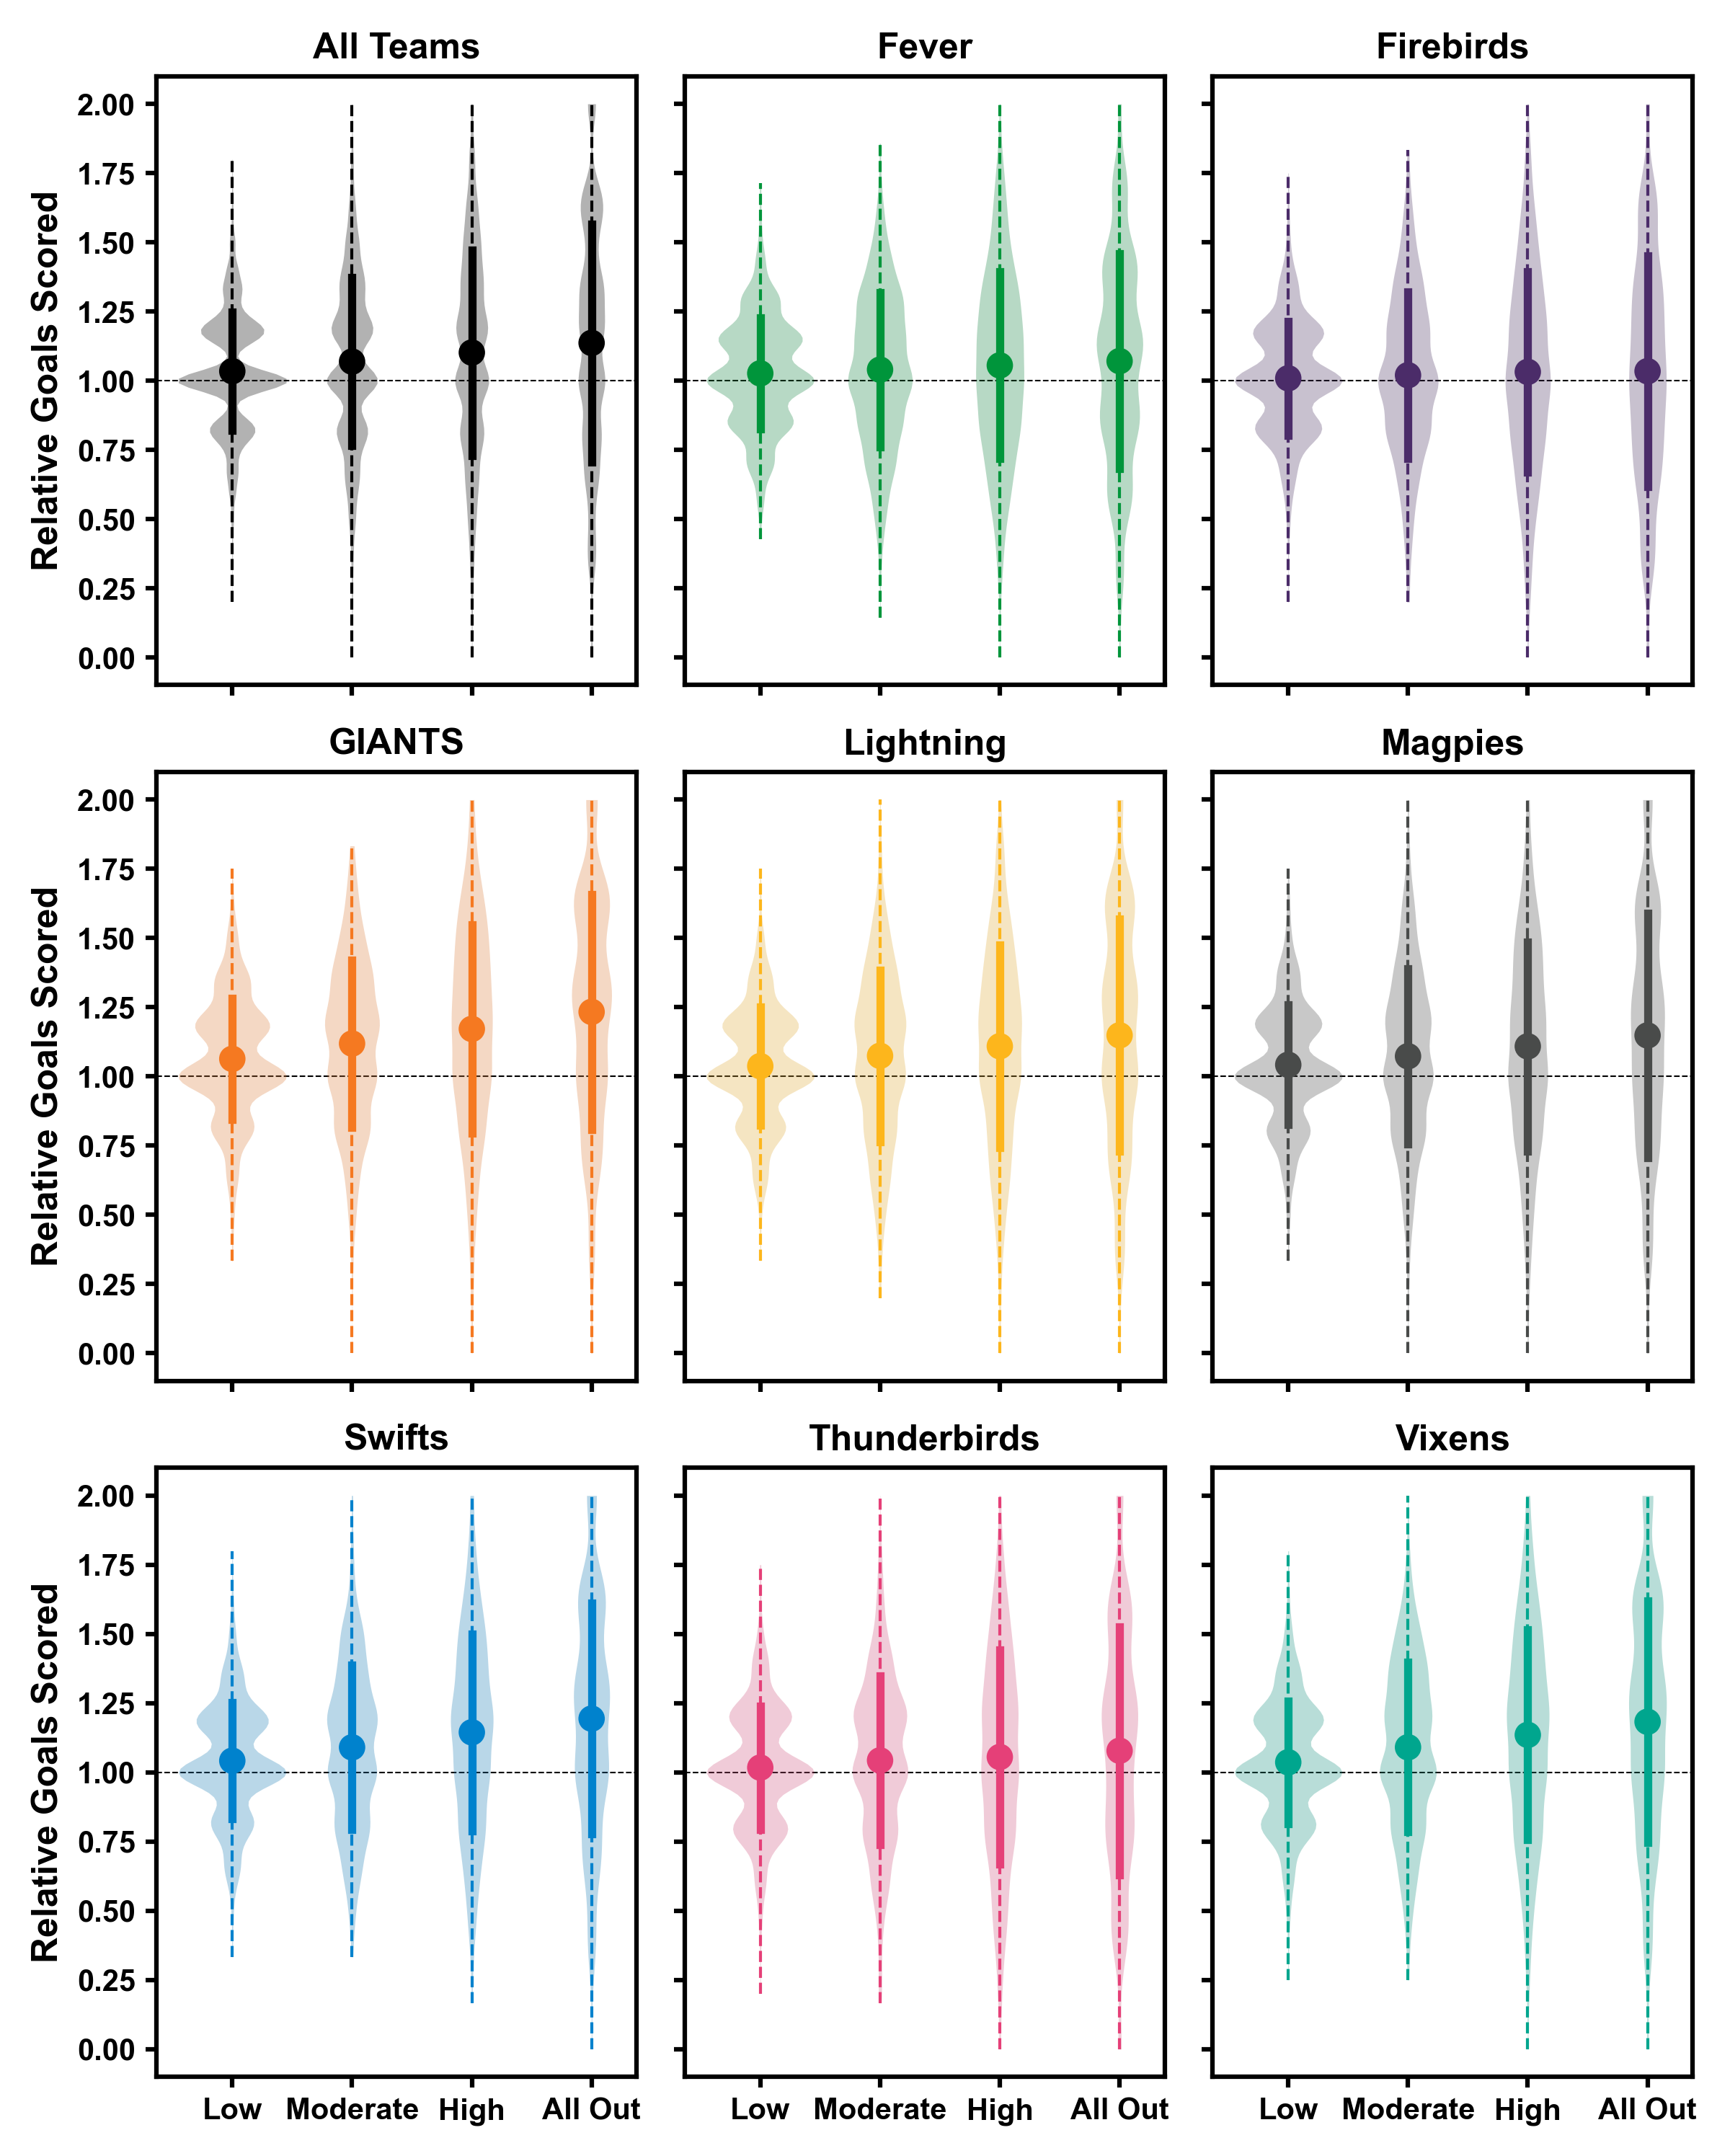
\includegraphics[width=1\linewidth]{C:/+GitRepos+/super-shot-sims/Results/standardSims/relativeGoalsScored} 

}

\caption{Total goals scored by teams across simulations (n = 1,000) with different Super Shot selection tendencies relative to the 'zero' Super Shot tendency. Point and solid lines represent mean $\pm$ standard deviation. Dashed line represents range of data. Shaded violin represents distribution of data.}\label{fig:standardSimsRelativeGoalsScored}
\end{figure}

Our simulations of Power 5 periods between teams revealed that on
average the margins between the two teams remained closed to zero
irrespective of the Super Shot tendency used or team involved (see
Figure \ref{fig:compSimsMarginFigure}). We observed larger vs.~smaller
maximal margins in simulation conditions where higher versus lower Super
Shot tendencies were simulated, respectively (see Figure
\ref{fig:compSimsMarginFigure}).

\begin{landscape}

\begin{figure}

{\centering 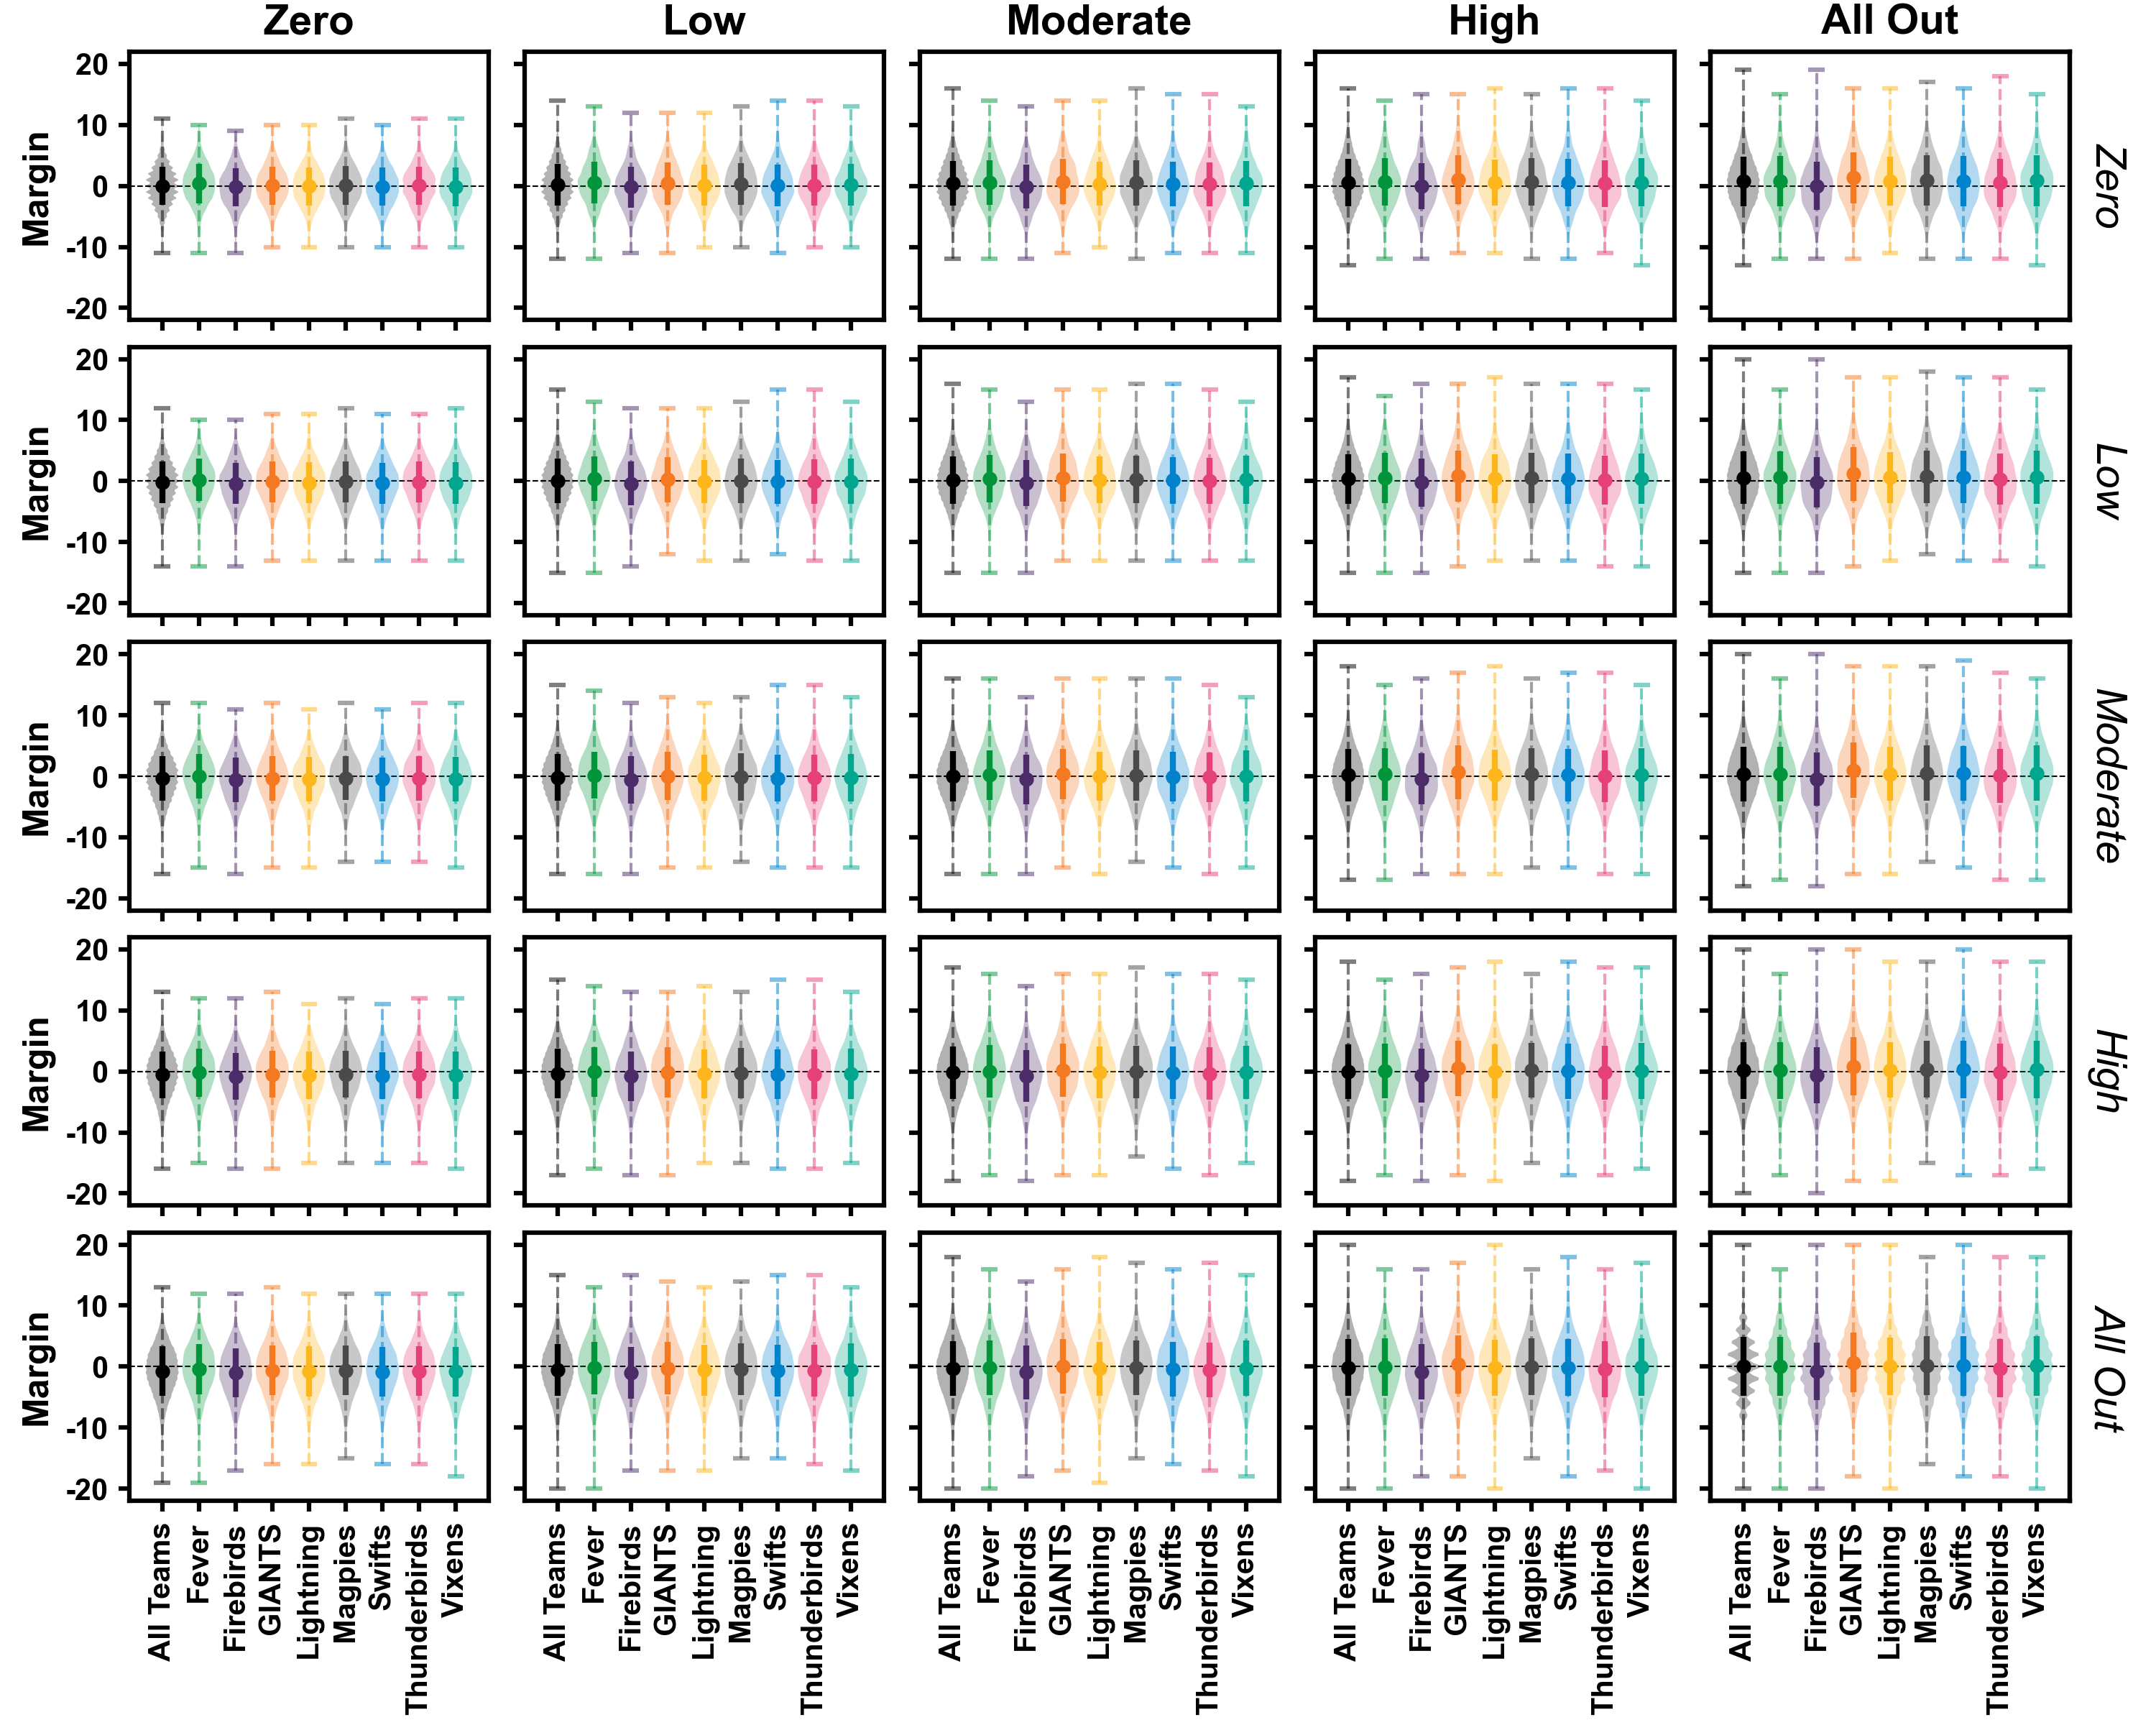
\includegraphics[width=1\linewidth]{C:/+GitRepos+/super-shot-sims/Results/compSims/compSimMargins} 

}

\caption{Power 5 period margin between teams during simulations (n = 1,000 using different Super Shot tendencies. Positive and negative margings reflect the period being won by the column-listed strategy (i.e. bolded) versus row-listed strategy (i.e. italicised), respectively. Point and solid lines represent mean $\pm$ standard deviation. Dashed line represents range of data. Shaded violin represents distribution of data.}\label{fig:compSimsMarginFigure}
\end{figure}

\end{landscape}

Supplementary figures\ldots{}

\hypertarget{discussion}{%
\section{Discussion}\label{discussion}}

\ldots{}

\begin{itemize}
\tightlist
\item
  Teams can score more with higher super shot tendencies, but also a lot
  less - larger ranges
\item
  In competitive sims, on average across large number of simulations
  things end up pretty even -- But there are some relatively clear
  floors and ceilings depending on strategies --- (e.g.~zero tendency
  vs.~all out, can't beat by as much as other strategies, and can also
  lose by a lot more)
\item
  While there weren't large fluctuations, certain teams had a better
  probability of winning a power 5 period with different strategies
\item
  Situational when to use
\item
  Conclusion - on average, it doesn't matter, but selection of Super
  Shot strategy likely needs to consider the situation, your teams
  skillset, and your opponents strategy
\end{itemize}

\ldots{}

Our analysis of shot statistics from the first season of the Super Shot
demonstrated an approximate four-times higher likelihood of missing from
the outer versus inner circle, irrespective of the match period
(i.e.~standard vs.~Super Shot period). While the 95\% CIs did overlap
between the two periods, a slightly higher risk of missing from the
outer versus inner circle was present in the Super Shot period. Our
present findings conflict with our earlier work from the 2018 Super
Netball season where we observed an approximate two-times higher risk of
missing from the outer versus inner circle --- and suggested that the
2:1 point ratio of the Super Shot represented `good' value relative to
the elevated risk of missing (\textbf{Fox2020?}). Our present analysis
perhaps suggests this is no longer the case --- as the risk of missing
from the outer circle has approximately doubled, and now outweighs the
additional point value on offer. Across the different teams and periods,
We found in all but one instance that the risk of missing from the outer
versus inner circle was greater than two-times that of the inner circle.
The only instance where the 95\% CIs overlapped the 2:1 ratio was for
the Firebirds during the standard period. This specific case is
irrelevant, however, as the additional points were not available during
this time. The obvious difference between the present study and our
previous work (\textbf{Fox2020?}) is the actual presence of the Super
Shot being on offer during the 2020 season. The elevated risk of missing
from the outer versus inner circle from the 2018 to 2020 Super Netball
season is similar to what we observed in originally comparing the 2018
Super Netball to Fast5 (i.e.~where long range shots were also rewarded
with additional points) (\textbf{Fox2020?}). Therefore, it seems
apparent that adding value to long-range shots in netball induces an
adjustment in the way either attacking and/or defensive teams play that
elevates the risk of missing long- versus close-range shots. There are a
number of factors that could be contributing to this elevated risk. The
most likely reason is an additional emphasis from defensive players on
preventing or contesting long-range shots given their added value. This
may also have an inverse effect on the difficulty of generating and
taking standard shot opportunities, where by virtue of defensive
strategies focusing on Super Shots could make it simpler for teams to
get easier shots closer to the post. The presence of the Super Shot may
also introduce psychological pressure on the shooting player and
influence the chance of success. A more thorough analysis of defensive
strategies and understanding shooting players perspectives around the
Super Shot can assist in understanding the mechanisms behind any
elevated risks of missing long-range shots with added rewards.

Despite the Super Shot potentially holding an unbalanced risk-reward
trade-off (in general), there are likely scenarios where it is an
attractive option or appropriate risk. When trailing by a large margin
with minimal time remaining, the one point on offer for a standard shot
may present very little value to the trailing team. In this scenario,
the Super Shot potentially becomes the only or default option.
Conversely, the leading team would likely adopt a `safe' approach and
minimise their Super Shot attempts. Our analysis also considered overall
team shooting statistics. The relative risk of missing a Super Shot may
change for an individual (i.e.~specialist) long-range shooter. If a team
possesses such a player, emphasising Super Shots could represent a
relatively valuable opportunity. Similarly, there is some evidence to
support the `hot-hand' premise in shooting sports
(\textbf{Bar-Eli2006?}). A team may benefit from preferentially feeding
a shooter possessing this characteristic for Super Shot attempts during
a Power 5 period.

Restricting Super Shot attempts appears to be a safe, but likely
limiting strategy for scoring during Power 5 periods. Our simulations
examining potential scoring outputs with varying Super Shot proportions
demonstrates this premise. Employing a low proportion (i.e.~\textless{}
30\%) of Super Shots resulted in relatively low to moderate, but
consistent, scoring outputs. The high probability of standard shot
success is the likely driving factor behind the consistent scoring with
lower Super Shot proportions (i.e.~higher standard shot proportions).
Conversely, a high proportion (i.e.~\textgreater{} 80\%) of Super Shots
resulted in a much wider spectrum of scoring outputs from relatively low
through to high. Increasing the proportion of Super Shots taken
generated a progressive increase in the maximum score achievable
(i.e.~higher ceiling), but also coincided with a decrease in the minimum
score achievable (i.e.~decreased floor). Teams taking a high proportion
of Super Shots during Power 5 periods likely expose themselves to
volatile scoring outcomes --- effectively `living or dying by the sword'
that is the Super Shot. \textbf{\emph{Anything to wrap-up this point?}}

Competitive simulation discussion paragraphs\ldots{}

Examining the `typical' margins within the simulated Power 5 periods
(i.e.~mean ± 95\% CIs) between teams revealed that, irrespective of the
strategies used, the margins were typically low -- rarely exceeding 1.5
to 2 points (see \ref{tab:marginTable}). There were times across the
simulations were higher margins were present (\textbf{\emph{TODO: refer
to supplementary figures}}), yet these were rarer occurrences. These
data suggest that optimising the proportion of Super Shots taken versus
allowing by a team and their opponent, respectively, can yield small but
potentially meaningful benefits. A yield of one to two goals across each
quarter would equate to four to eight goals across an entire match.
Given netball matches can often be decided by a small number of goals --
this may present a significant advantage for a team. There is, however,
a degree of variability across these results and teams would not be able
to expect the same outcome every time a specific strategy is employed.
This would likely be more evident with respect to strategies employing a
high propotion of Super Shots. As identified in our earlier analyses, a
higher proportion of Super Shots introduces a degree of volatility in a
teams scoring output -- and hence has the same potential to introduce
volatility in the margin the team would encounter during such Power 5
periods.

\ldots high proportion of Super Shots may yield a beneficial result on
average for a team, but given the approach being taken there will likely
be times where this could backfire on the team\ldots{}

The optimal proportion of Super Shots to take versus allow likely varies
from team to team. For example, \ldots{}

\ldots also other factors to consider that may dictate
success\ldots number of shots\ldots shooting percentage\ldots{} For
example, generating a greater number of shot opportunities than your
opponent will likely lead to better scoring and margins - and may also
provide a greater scope to risk taking a greater number of Super
Shots\ldots{} \ldots investigating these additional
factors\ldots outside the scope of this investigation\ldots{}

Looking at the margin summaries (mean +/- 95\% CI's) from each teams
competitive simulations across all opponents, certain strategies
appeared more or less favourable across different teams. For example,
where the Fever extended above 50\% of their shots as Super Shots, it
was typical for them to score less than their opponent in the Super Shot
period; whereas when they used no Super Shots they typically outscored
their opponents. Other trends\ldots?

Remaining discussion points\ldots{}

Our approach in the present paper to simulate Super Shot scoring periods
differs to our original work (\textbf{Fox2020?}). Previously, we
allocated an overall success rate to shots from the inner versus outer
circle (i.e.~if the sampled probability was 50\%, a total of 50\% of
shots were counted as successful). This contrasts to our present work,
where we sampled and applied the probability of shot success to
simulated individual shots (i.e.~if the sampled probability is 50\%, the
individual shot being simulated has a 50\% probability of success). This
approach likely reflects an improvement on our analysis, better
representing the independent nature of shots in a netball match.

\begin{itemize}
\tightlist
\item
  Team specific values, any obvious differences? For example, one team
  may have had better success and therefore using a higher proportion in
  general may have led to higher percentage of `won' periods
\item
  Team vs.~team specific values and if they are different across various
  opponents. For example, better shooting success with high super shot
  proportions vs.~one team but not another? This may be more relevant if
  we use opponent specific probabilities of super shot success.
  Important that the lack of `defensive' presence within simulations is
  acknowledged as a limitation, in that we applied the same super shot
  probability rates for each team from their entire season, rather than
  individually vs.~their oposition team. Given we might have some
  relative risk of missing against different defensive opponents, this
  may actually reveal that this should be a consideration if one team is
  more effective with their defense
\item
  Practical considerations of work include strategising around super
  shot, with respect to how many to take perhaps depending on margin
  along with opposition, as well as own teams success in this realm
\end{itemize}

Discussion notes\ldots check paragraphs here

Our simulation data does, however, demonstrate potential value in using
the Super shot for certain teams and in certain scenarios. Times where
higher proportion of super shot was valuable? We incorporated variable
shot opportunity numbers based on league data, and hence the number of
shot opportunities varied across individual simulations for teams. This
was balanced, in that when teams received more shot opportunities, their
opposition received fewer. Across all simulations, the wining team
received more shots on x\% of times. This factor became more/less
evident across scenarios where a team took a higher proportion of super
shots, whereby the winning team had more shots in x\% of these
simulations. This firstly suggests that generating more shot
opportunities than your opponent is obviously beneficial, but
potentially awards you more flexibility when considering taking a
greater proportion of super shots.

Similarly, teams who were better with the Super shot fared better in
simulations with greater proportions of super shots, and vice versa for
teams that are worse. For example, the fever lost x\% of simulations
when they went heavy on the Super shot, vs.~X team who won x\% of
simulations when using a high \% proportion of super shots. This is not
surprising as the fever had the highest risk of missing from the outer
vs inner circle, particularly during Super shot periods. These findings
likely demonstrate a need for teams to play to their shooting strengths.

\hypertarget{conclusion}{%
\section{Conclusion}\label{conclusion}}

\ldots{}

Scenario specific use\ldots{}

Limitations - global probability of Super Shot success from teams across
three seasons, unlikely to be representative of the exact shooting
combinations that are put forward during a Power 5 period (e.g.~emphasis
may be given to specialist long distance shooter); independent
probability approach whereby each individual shot was pitted against
overall probability of success (i.e.~ignores any sort of `hot hand'
effect); similarly, the tendencies simulated were all or nothing in a
sense that in an `All Out' strategy if the first couple of Super Shots
missed the team might pull back, hence some simulations likely
represented worst case outcomes that may not eventuate in such a
circumstance

\hypertarget{bibliography-styles}{%
\section{Bibliography styles}\label{bibliography-styles}}

There are various bibliography styles available. You can select the
style of your choice in the preamble of this document. These styles are
Elsevier styles based on standard styles like Harvard and Vancouver.
Please use BibTeX~to generate your bibliography and include DOIs
whenever available.

Here are two sample references: (Dirac, 1953; Feynman and Vernon Jr.;
1963).

\hypertarget{references}{%
\section*{References}\label{references}}
\addcontentsline{toc}{section}{References}

\hypertarget{refs}{}
\begin{CSLReferences}{1}{0}
\leavevmode\vadjust pre{\hypertarget{ref-Dirac1953888}{}}%
Dirac, P.A.M., 1953. The lorentz transformation and absolute time.
Physica 19, 888--896.
doi:\href{https://doi.org/10.1016/S0031-8914(53)80099-6}{10.1016/S0031-8914(53)80099-6}

\leavevmode\vadjust pre{\hypertarget{ref-Feynman1963118}{}}%
Feynman, R.P., Vernon Jr., F.L., 1963. The theory of a general quantum
system interacting with a linear dissipative system. Annals of Physics
24, 118--173.
doi:\href{https://doi.org/10.1016/0003-4916(63)90068-X}{10.1016/0003-4916(63)90068-X}

\end{CSLReferences}


\end{document}
